\documentclass[]{spie}  %>>> use for US letter paper
%\documentclass[a4paper]{spie}  %>>> use this instead for A4 paper

\renewcommand{\baselinestretch}{1.0} % Change to 1.65 for double spacing

\usepackage{amsmath,amsfonts,amssymb}
\usepackage{graphicx}
\usepackage[colorlinks=true, allcolors=blue]{hyperref}
\usepackage{xcolor}
\usepackage{float}
\usepackage{booktabs}
\usepackage{enumitem}

\graphicspath{{../figures/}}

\newcommand{\degC}{$^{\circ}$C}

% AAS journal abbreviations used by ref.bib (matching aastex/AASTeX conventions)
\newcommand{\pasp}{Publ. Astron. Soc. Pac.}
\newcommand{\apj}{Astrophys. J.}
\newcommand{\apjl}{Astrophys. J. Lett.}
\newcommand{\apjs}{Astrophys. J. Suppl. Ser.}
\newcommand{\aap}{Astron. \& Astrophys.}
\newcommand{\aaps}{Astron. \& Astrophys. Suppl. Ser.}
\newcommand{\mnras}{Mon. Not. R. Astron. Soc.}
\newcommand{\aj}{Astron. J.}
\newcommand{\nat}{Nature}
\newcommand{\araa}{Annu. Rev. Astron. Astrophys.}

\title{Precision twilight forecasting for dome seeing mitigation at the Vera C. Rubin Observatory}

\author[a]{Johnny~H.~Esteves}
\author[a]{Christopher~W.~Stubbs}
\affil[a]{Department of Physics, Harvard University, Cambridge, MA 02138, USA}

\authorinfo{Send correspondence to J.H.E.: E-mail: jesteves@fas.harvard.edu}

% Option to view page numbers
\pagestyle{empty} % change to \pagestyle{plain} for page numbers
\setcounter{page}{1}

\begin{document}
\maketitle

\begin{abstract}
Precise thermal control is a prerequisite for the Vera C. Rubin Observatory to meet the image-quality requirements of the Legacy Survey of Space and Time (LSST), since temperature differentials between the combined primary/tertiary mirror (M1M3), dome air, and ambient environment drive both dome seeing and mirror seeing. We present NBEATSx+Ridge, a two-stage causal forecasting architecture that predicts twilight temperature on a uniform solar-time grid using only past local observations. The first stage (NBEATSx, a deep learning model) captures nonlinear temporal dynamics; the second stage (Ridge regression) corrects systematic biases using engineered features evaluated at the forecast issuance time. Evaluated on 396 twilight events in 2025 with strictly causal training (pre-2025 data only), the system achieves RMSE of 0.80\degC{} at the operationally critical 3\,h lead time (dome opening), with 80\% of predictions within 1\degC{}---compared with the $\sim$2\degC{} residual scatter that the bias-corrected MeteoBlue NWP forecast retains at this site. We further propose a three-phase thermal-control scheme for M1M3 that consumes these forecasts, and use an end-to-end simulation to show how upstream forecast skill would translate into mirror-temperature regulation for the Rubin thermal system.
\end{abstract}

\keywords{Image quality, dome seeing, thermal control, time-series forecasting, deep learning, NBEATSx, Rubin Observatory, LSST}

%% =============================================================
\section{INTRODUCTION}
\label{sec:intro}

The performance of ground-based optical observatories depends critically on image quality and thermal control. One key challenge is \emph{dome seeing}, which arises from temperature gradients between the interior and exterior of the telescope enclosure.\cite{Racine1991, Emelianov2015} Dome air conditioning (HVAC) systems reduce these gradients by matching the internal air temperature to the outside ambient temperature. However, the effectiveness of this pre-cooling strategy depends on anticipating the outside temperature well in advance---most critically during the twilight transition when the dome is first opened and the massive thermal inertia of the telescope structure makes maintaining thermal equilibrium particularly difficult.

For the Vera C. Rubin Observatory,\cite{ivezic19} this challenge is magnified because the LSST requires rapid data acquisition and exceptionally consistent image quality across a wide field of view.\cite{Esteves2023} Rubin employs a Ventilation and Air Conditioning (HVAC) system that actively preconditions the enclosure and mirror to track the outside temperature. The operational efficiency of this active control system depends on precise forecasts of the outside air temperature. Figure~\ref{fig:dataset_overview} shows a representative year of summit temperature data, the twilight transitions our forecasts target, and the half-solar-day differenced signal that motivates the model architecture introduced below.

Traditional NWP models from ECMWF, GFS, or commercial services like MeteoBlue struggle with site-specific predictions at high-altitude sites like Cerro Pach\'on due to coarse spatial resolution and inadequate boundary layer parameterizations. Following Buffa et~al.,\cite{Buffa1997} who demonstrated neural networks for dome temperature prediction, the Rubin Observatory deployed a Prophet-based\cite{Taylor2017} forecasting system using local weather station data. While this eliminated global forecast biases, higher precision is required for autonomous thermal control.

\begin{figure}[htb!]
    \centering
    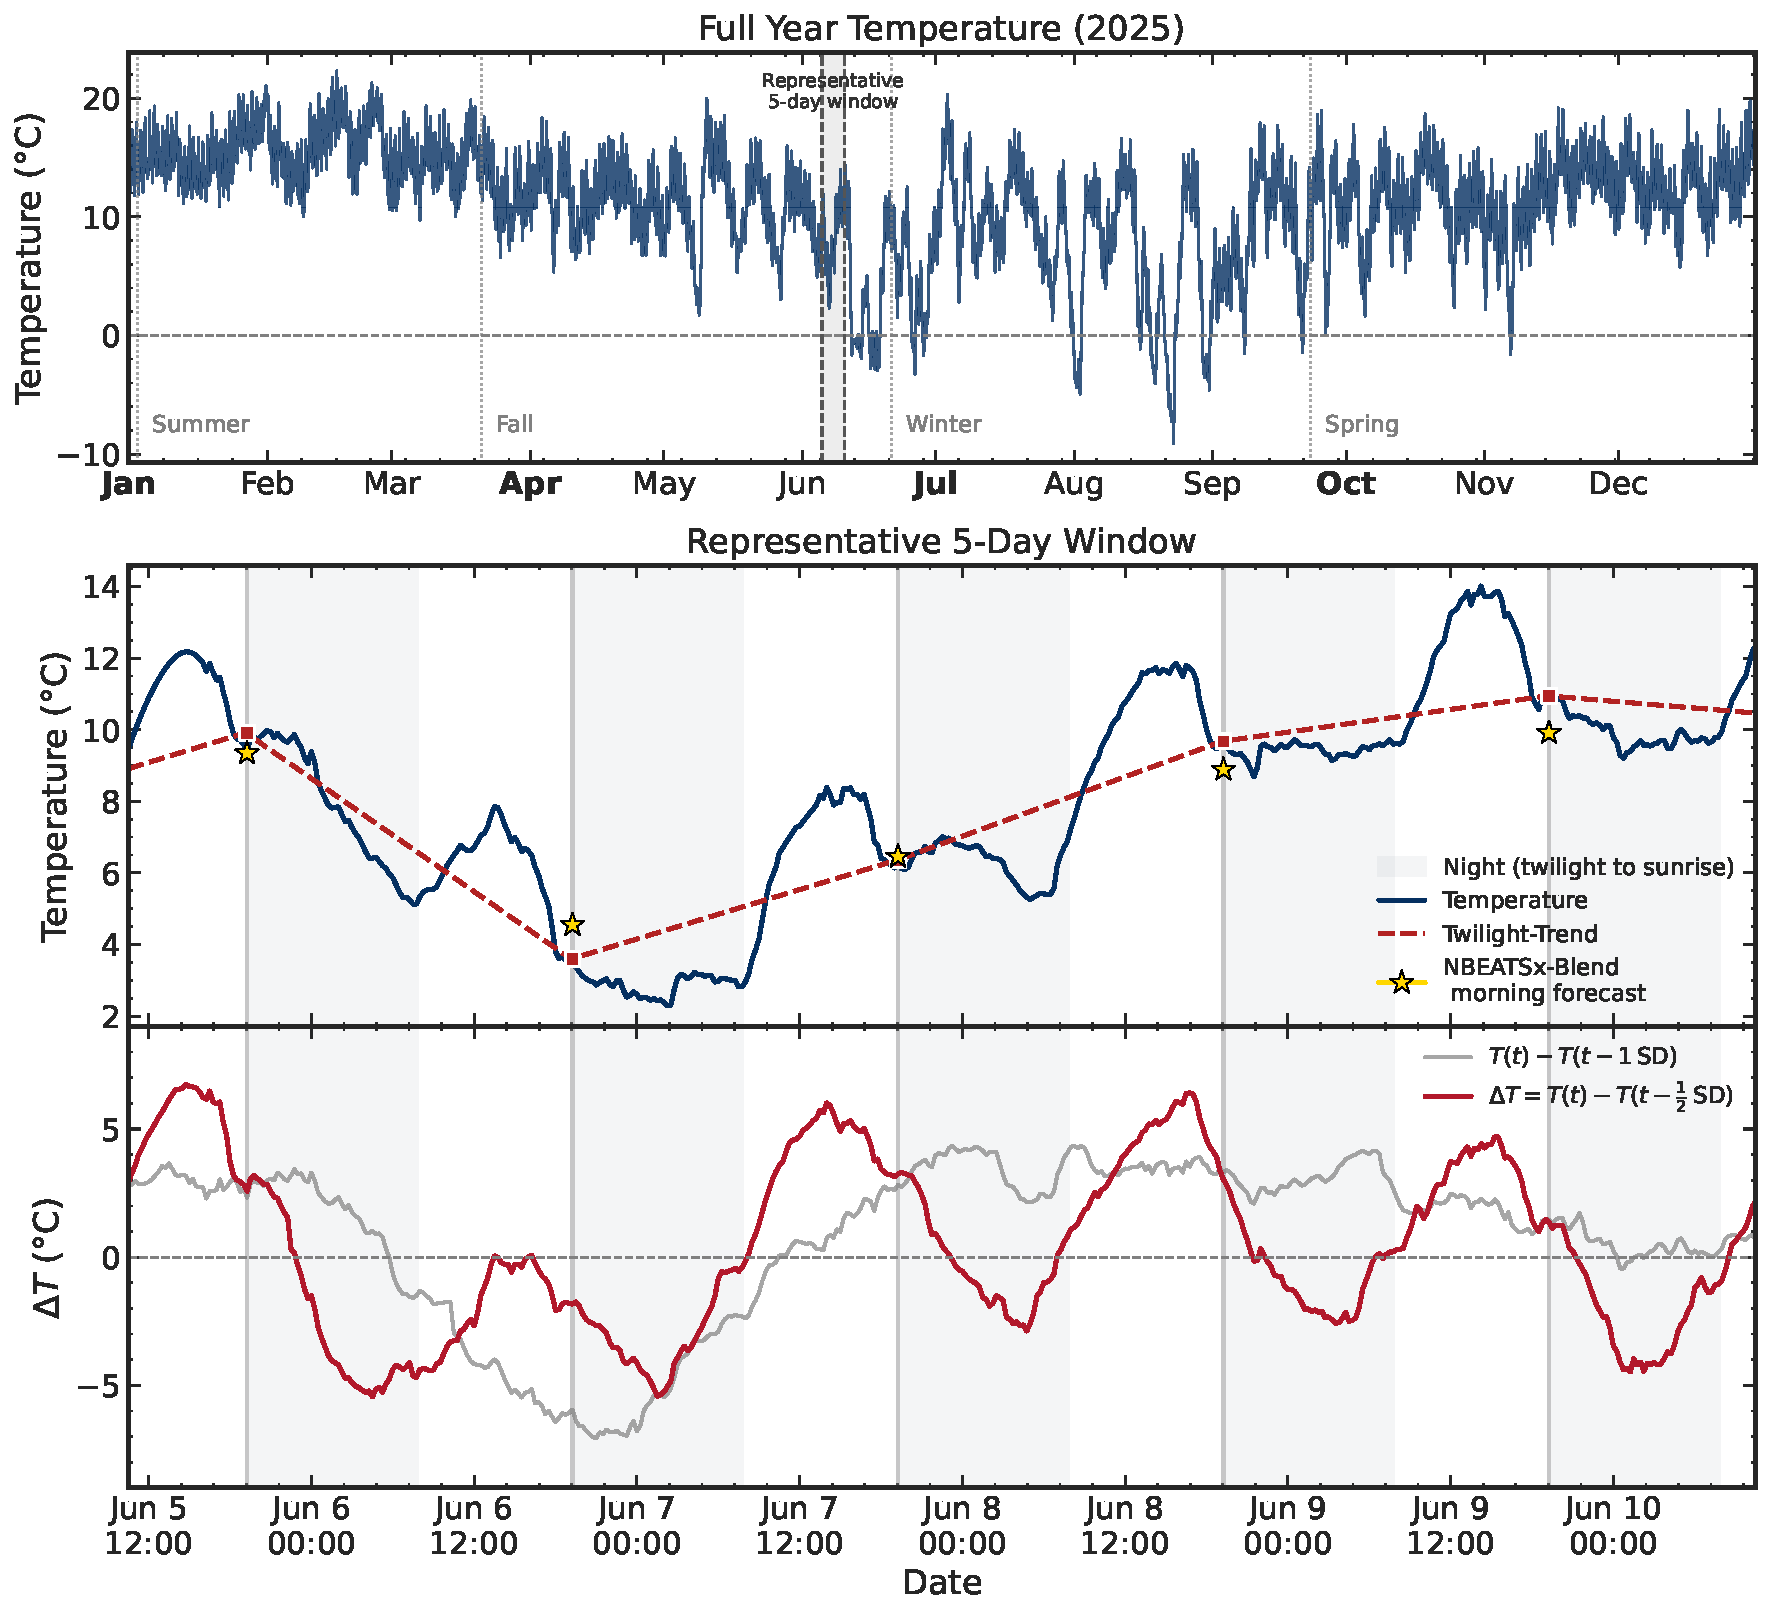
\includegraphics[width=0.95\textwidth]{fig0_dataset_overview.pdf}
    \caption{Dataset overview. \textbf{Top:} Full year of ambient temperature data (2025) from the Cerro Pach\'on summit weather tower. \textbf{Middle:} Detailed 5-day window showing the diurnal cycle and twilight events (gray vertical lines). Gold stars show NBEATSx+Ridge forecasts issued at midday. Note the strong afternoon cooling on Jun~6, representative of synoptic-scale weather passages that challenge all forecast models. \textbf{Bottom:} Differenced signals used as diagnostic features. The gray curve $T(t) - T(t-1\,\text{SD})$ captures day-to-day synoptic changes; the red curve $\Delta T = T(t) - T(t - \frac{1}{2}\,\text{SD})$ has reduced amplitude because the 12-hour lag aligns similar phases of the diurnal cycle.}
    \label{fig:dataset_overview}
\end{figure}

In this work, we present NBEATSx+Ridge, a two-stage causal forecasting architecture that predicts twilight temperature on a uniform solar-time grid using only past local observations. The first stage (NBEATSx\cite{Olivares2021}) captures nonlinear temporal dynamics; the second stage (Ridge regression) corrects systematic biases using engineered features. We compare against Persistence, Linear Regression, Random Forest, and MLP baselines, demonstrating that NBEATSx+Ridge achieves the best performance across all forecast horizons from 0.5 to 12 hours.

%% =============================================================
\section{DATA ACQUISITION AND PRE-PROCESSING}
\label{sec:data}

\subsection{Site and instrumentation}
\label{sec:data:site}

The forecast system utilizes historical and real-time data from the Summit Weather Tower temperature sensor located at the Vera C. Rubin Observatory on Cerro Pach\'on ($30.2^\circ$S, $70.7^\circ$W, 2663\,m elevation). The data span approximately 3 years (2022--2025), providing a robust historical baseline for training (Fig.~\ref{fig:dataset_overview}).

\subsection{Data cleaning and noise characterization}
\label{sec:data:cleaning}

Raw telemetry from the LSST Engineering and Facility Database (EFD) is resampled from 1-minute to 15-minute intervals using the mid-range mean $(T_{\text{max}} + T_{\text{min}})/2$. The Summit Weather Tower sensor (Young Model 41382VC in a multi-plate radiation shield) exhibits two distinct noise regimes: a stable nighttime floor of $\sigma \approx 0.12$\degC{}, and elevated daytime noise ($\sigma \approx 0.23$\degC{}) caused by solar-induced convective turbulence in the radiation shield at high solar altitudes. Points with intra-interval spread exceeding 3\degC{} are replaced using causal forward-fill. For forecast evaluation, validation actuals at twilight are computed from a 3-hour Gaussian-smoothed temperature series (centered, $\sigma = 2$ grid steps), which suppresses sensor jitter while preserving the true ambient temperature signal at the $\sim$30-minute timescale relevant for thermal control. This window is also comparable to the mirror/dome thermal response time ($\tau \approx 3$\,h; Sec.~\ref{sec:thermal}), so the smoothed series reflects the temperature the thermal system physically integrates rather than sensor jitter.

\subsection{Solar-time grid}
\label{sec:data:solar_grid}

Rather than operating on a fixed clock-time grid, we resample all data onto a \emph{uniform solar-time grid} with 48 steps per solar day. We define a normalized solar time $\phi \in [0,1)$ anchored to local sunrise and sunset:
\begin{equation}
\phi = \begin{cases}
\displaystyle \frac{1}{2}\,\frac{t - t_{\text{sunrise}}}{t_{\text{sunset}} - t_{\text{sunrise}}} & \text{(daytime)} \\[8pt]
\displaystyle \frac{1}{2} + \frac{1}{2}\,\frac{t - t_{\text{sunset}}}{t_{\text{sunrise,next}} - t_{\text{sunset}}} & \text{(nighttime)}
\end{cases}
\label{eq:solar_time}
\end{equation}
where $\phi = 0$ at sunrise, $\phi = 0.25$ at solar midday, $\phi = 0.5$ at sunset, and $\phi = 0.75$ at solar midnight. One ``solar day'' (SD) spans from sunrise to the next sunrise ($\phi: 0 \to 1$). Daytime is normalized by the actual day length and nighttime by the actual night length, so that diurnal landmarks always occur at fixed grid positions regardless of season. A monotonically increasing coordinate $\phi_{\text{abs}} = N_{\text{day}} + \phi$ (where $N_{\text{day}}$ increments at each sunrise) provides the uniform sampling axis. Resampling the 15-minute telemetry onto this grid at 48 steps/SD ($\Delta\phi = 1/48$) yields a $\sim$30-minute equivalent cadence where lag features have consistent physical meaning year-round. An ablation that re-runs the identical NBEATSx+Ridge pipeline on a fixed clock-time grid confirms the benefit is real but mild ($\sim$6\% RMSE improvement), as seasonal day-length variation otherwise misaligns clock-time lags.

\subsection{Train/test split strategy}
\label{sec:data:split}

All models are trained on data prior to January 1, 2025, and evaluated on all 396 twilight events in 2025. NBEATSx uses an additional 10\% validation holdout from the training period for early stopping. Baseline models (Linear, Random Forest, MLP) are trained per lead time using the same temporal split.

%% =============================================================
\section{METHODS}
\label{sec:methods}

\subsection{Persistence baseline}
\label{sec:methods:persistence}

The simplest sensible forecast is persistence on the diurnal cycle: use \emph{yesterday's temperature at the same time} as today's prediction. This is cheap and assumption-free, and already achieves $\sim$2.8\degC{} RMSE at twilight---most of the diurnal signal is captured simply because the day-night cycle repeats. We sharpen this idea with a \emph{solar-persistence} baseline that exploits the regularity of the diurnal cycle on the solar-time grid:
\begin{equation}
\hat{T}_{\text{persist}}(\phi_{\text{tw}}) = T(\phi_{\text{now}}) + \left[ T(\phi_{\text{tw}} - 1\,\text{SD}) - T(\phi_{\text{now}} - 1\,\text{SD}) \right]
\label{eq:persistence}
\end{equation}
This predicts that today's temperature change from now to twilight will equal yesterday's change over the same solar-time interval. Equivalently, it assumes $\Delta T(\phi) = T(\phi) - T(\phi - 1\,\text{SD}) \approx \text{const}$ over one day---i.e., persistence on the day-to-day difference. This baseline is non-trivial: because the solar grid aligns diurnal landmarks, ``same time yesterday'' genuinely corresponds to the same physical regime (same solar heating geometry, same phase of the cooling curve). It achieves RMSE of 1.19\degC{} at 3h lead---already a strong forecast that all learned models must beat. Its skill is governed by the stability of the day-to-day difference: if the day-to-day variation is constant (grey curve in Fig.~\ref{fig:dataset_overview}, $T(t)-T(t-1\,\text{SD})$), then ``same solar time yesterday'' is an excellent proxy; the baseline degrades only when this difference shifts sharply between successive days (Sec.~\ref{sec:results:seasonal}).

\subsection{Prophet}
\label{sec:methods:prophet}

Prophet\cite{Taylor2017} is a time-series model that decomposes the signal into trend, seasonality, and holiday components using a generalized additive model with piecewise-linear or logistic growth. We deploy a hybrid configuration (Prophet-BMA) that fits separate short-term and long-term Prophet models with a 7-day training window, then blends their predictions using Bayesian Model Averaging with exponential weighting $\alpha(h) = 0.9 \cdot e^{-h/13}$, giving the short-term model dominance at small lead times while transitioning to the more stable long-term model at longer horizons. This was the operational forecast at Rubin Observatory prior to this work.

\subsection{Supervised baselines: Linear, Random Forest, MLP}
\label{sec:methods:baselines}

These three models predict the absolute twilight temperature $T(\phi_{\text{tw}})$ directly from a feature vector computed at forecast issuance time $\phi_{\text{now}}$. A separate model is trained for each lead time $h$, with features extracted on the solar grid:
\begin{itemize}[noitemsep]
    \item $y_{\text{raw}}$: current temperature $T(\phi_{\text{now}})$
    \item $y_{\text{lag-6}}, y_{\text{lag-12}}, y_{\text{lag-24}}, y_{\text{lag-48}}$: temperatures at 3h, 6h, 12h, and 24h before $\phi_{\text{now}}$
    \item trend\_solar\_2h: backward OLS slope over 4 grid steps ($\sim$2h)
    \item $\sin/\cos(\phi)$, $\sin/\cos(\text{doy})$: deterministic solar-time and seasonal phase
\end{itemize}

\noindent\textbf{Linear:} Ridge-regularized regression ($\alpha = 1.0$), features standardized.\\
\textbf{Random Forest:} 100 trees, max depth 10, min 5 samples per leaf, no standardization.\\
\textbf{MLP:} Two hidden layers (64, 32 units), ReLU activation, learning rate $10^{-3}$, early stopping, max 1000 iterations, features standardized.

All three models are trained on pre-2025 data and evaluated on 396 twilights in 2025. Because each model is trained per lead time, it learns the specific relationship between features at that horizon and the twilight target---effectively learning the expected temperature change as an implicit function of the inputs.

\subsection{NBEATSx+Ridge: two-stage architecture}
\label{sec:methods:nbeatsx}

We employ a two-stage forecasting architecture. The first stage uses NBEATSx\cite{Olivares2021} (an extension of N-BEATS\cite{Oreshkin2020} with exogenous variables) to predict the absolute twilight temperature directly. The second stage applies a Ridge regression correction that combines the NBEATSx prediction with engineered features to remove systematic biases.

\paragraph{Stage 1: NBEATSx (direct-$T$).}
NBEATSx\cite{Olivares2021} predicts $\hat{T}_{\text{NB}}(\phi_{\text{tw}})$ from a 48-step lookback window using four specialized stacks (trend, seasonality, identity, exogenous), each with one block of width 16. Historical features: $y_{\text{raw}}$, $y_{\text{lag-24}}$, trend\_solar\_2h, and $y_{\text{diff-24h}}$; future features: $\sin/\cos$ of solar time and day-of-year. Trained on $\sim$20\,000 pre-2025 grid rows for 700 steps (SELU, Huber loss, early-stopping patience 10). The small width was selected by sweep: larger networks overfit on this training volume.

\paragraph{Stage 2: Ridge correction.}
The NBEATSx prediction $\hat{T}_{\text{NB}}$ is combined with a richer feature vector evaluated at the forecast issuance time to produce the final forecast:
\begin{equation}
\hat{T}_{\text{final}}(h) = \text{Ridge}\bigl(\mathbf{x}(\phi_{\text{now}}),\; \hat{T}_{\text{NB}}(\phi_{\text{tw}})\bigr)
\label{eq:ridge}
\end{equation}
where $\mathbf{x}$ contains 13 solar-grid features (the 10 Linear-baseline features plus trend\_solar\_4h, velocity\_noon, and dmean\_1d---selected by greedy forward sweep). At long leads ($\geq$5\,h) this set is augmented with multi-day trend, humidity, and direction-resolved wind features that reduce the Winter/Spring morning-forecast error (Sec.~\ref{sec:results:seasonal}); the augmented features are withheld at short lead, where they would only add estimation variance. A separate Ridge model is fit per lead. Ridge is trained on pre-2025 twilight events using the NBEATSx in-sample predictions; it is evaluated on 2025 twilights using the NBEATSx out-of-sample predictions. This separation ensures strict temporal causality: the Ridge stage never sees 2025 data during training.

The two-stage design exploits complementary strengths: NBEATSx captures nonlinear temporal dynamics from the contiguous time series, while Ridge provides stable, feature-driven bias correction calibrated on twilight events. Neither stage alone matches the combined RMSE of 0.80\degC{} at 3\,h.

%% =============================================================
\section{TWILIGHT FORECAST VERIFICATION}
\label{sec:verification}

\subsection{RMSE by model and lead time}
\label{sec:results:rmse}

Figure~\ref{fig:rmse_vs_lead} presents the RMSE for all models across lead times from 0.5 to 12 hours, with shaded bands indicating 95\% bootstrap confidence intervals. NBEATSx+Ridge consistently achieves the lowest RMSE at horizons beyond 1 hour. At short lead times ($<$1h), all learned models converge to $\sim$0.3--0.5\degC{} as the prediction horizon shrinks toward zero. The solar-persistence baseline (Eq.~\ref{eq:persistence}) grows steadily from $\sim$0.5\degC{} at 0.5h to $\sim$1.8\degC{} at 12h, reflecting the increasing difficulty of assuming today matches yesterday as the forecast window widens.

\begin{figure}[htb!]
    \centering
    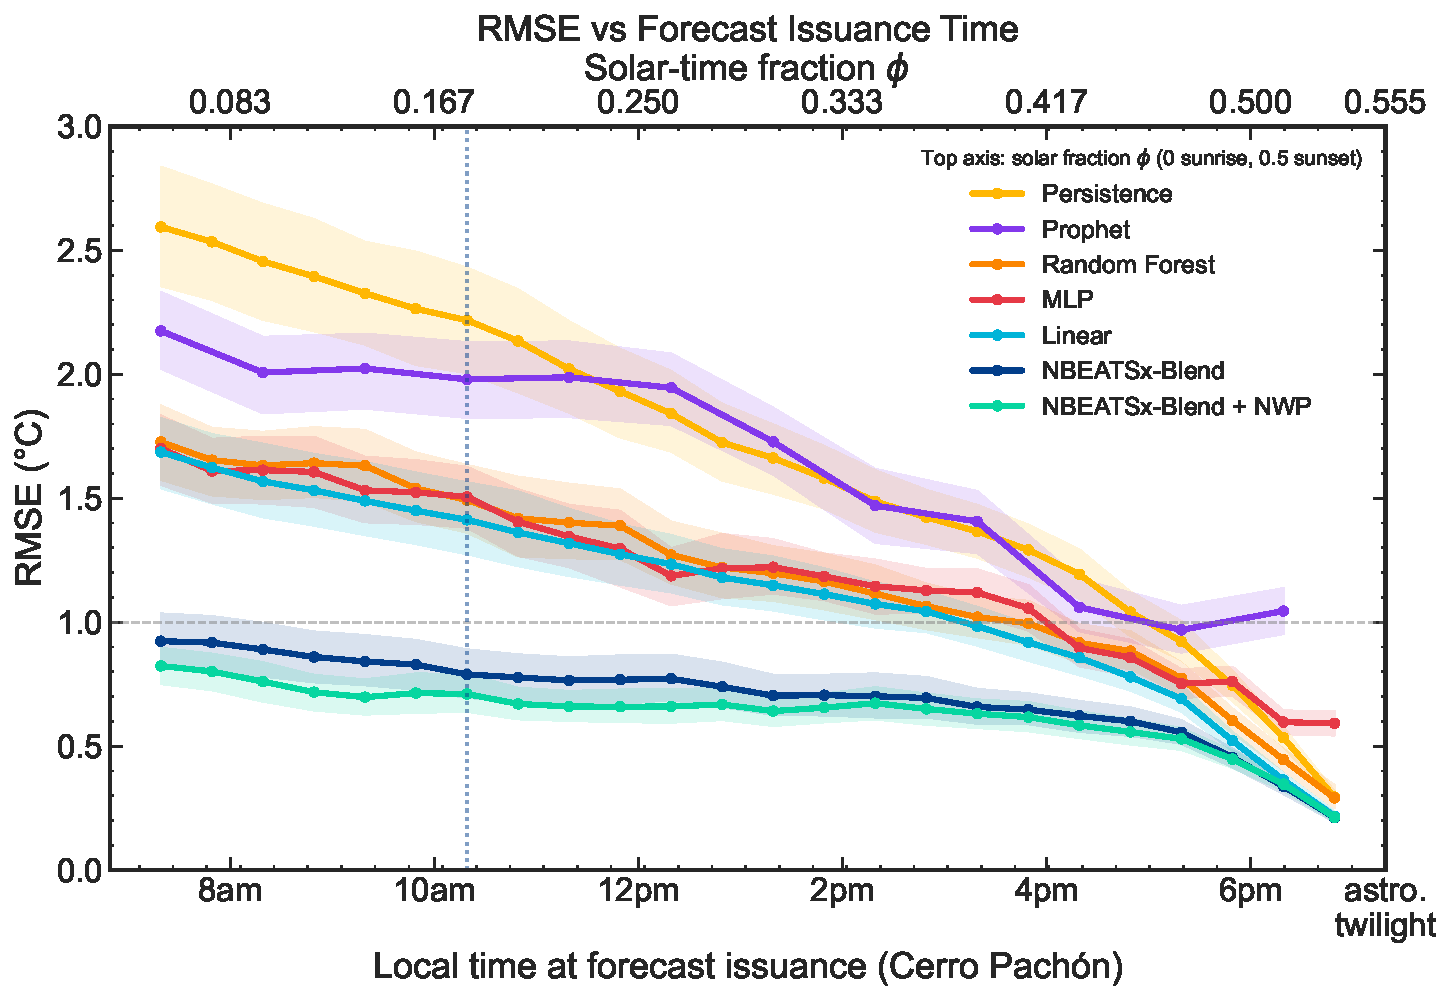
\includegraphics[width=0.85\textwidth]{fig3_rmse_vs_lead_time.pdf}
    \caption{RMSE as a function of forecast issuance time with 95\% bootstrap confidence bands. The bottom axis labels are equivalent local clock time at Cerro Pach\'on \emph{on the equinox} (sunrise $\approx$ 6\,am, sunset $\approx$ 6\,pm, astronomical twilight $\approx$ 7:20\,pm); the top axis is the solar-time fraction $\phi$ used throughout this paper, valid year-round, with $\phi=0$ at sunrise, $0.5$ at sunset, and the forecast target (astronomical twilight, $\mathrm{alt}_\odot = -20^\circ$) at $\phi \approx 0.555$. NBEATSx+Ridge (dark navy) achieves the lowest RMSE across all horizons. Solar-persistence (gold) provides a strong non-trivial baseline that grows steadily with lead time as day-to-day variability accumulates. The vertical dotted line marks the operationally critical lead at which the M1M3 mirror-control setpoints are issued ($\sim$3\,h before twilight, $\sim$4\,pm equivalent); the horizontal dashed line indicates the 1\degC{} target.}
    \label{fig:rmse_vs_lead}
\end{figure}

\subsection{Current state: external operational forecasts}
\label{sec:results:comparison}

Before isolating performance at the operationally critical lead, it is useful to anchor the discussion against the forecasts already available at Rubin. Figure~\ref{fig:comparison} compares NBEATSx+Ridge, the Prophet-based operational forecast, and the MeteoBlue commercial NWP service at the 6-hour (midday) lead time. NBEATSx+Ridge demonstrates superior performance: tighter scatter around the 1:1 line, near-unity slope, and minimal systematic bias. MeteoBlue alone suffers from large systematic bias at this high-altitude site, reflecting the limited spatial resolution of global NWP models. The Prophet-based system, while unbiased, exhibits substantially larger scatter than the deep learning approach.

\begin{figure}[htb!]
    \centering
    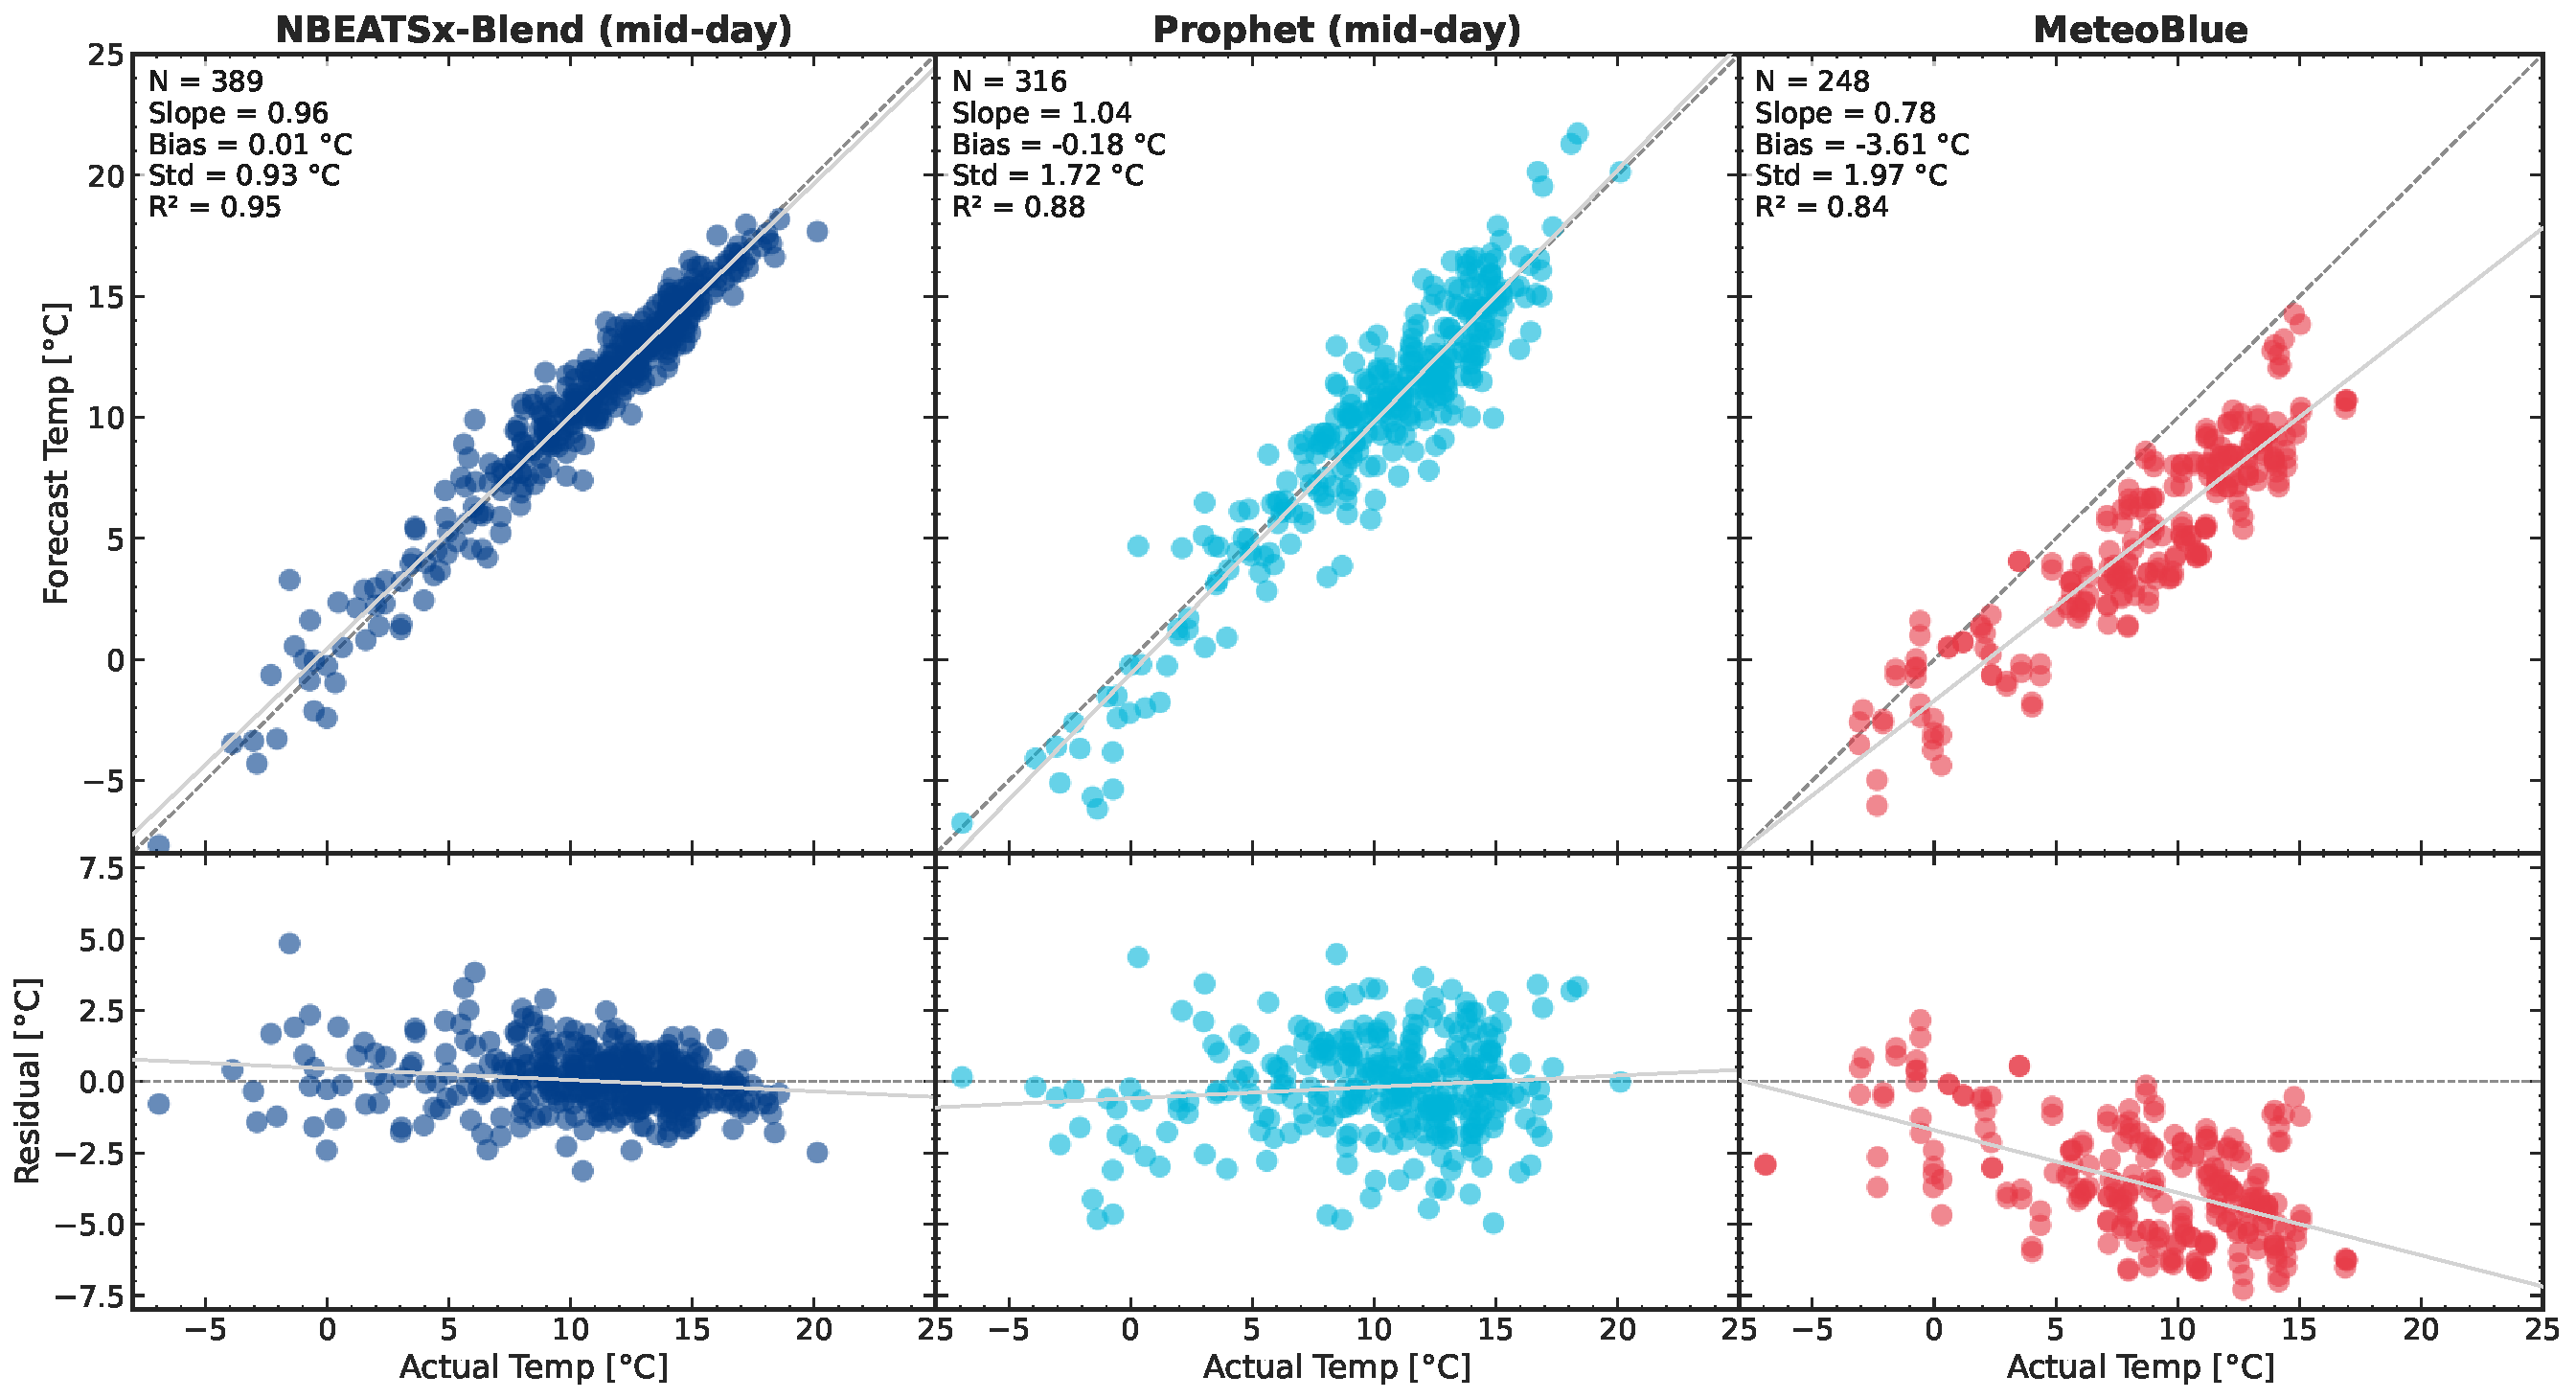
\includegraphics[width=\textwidth]{fig8_comparison.pdf}
    \caption{Comparison of twilight temperature forecasts at midday (6-hour lead). \textbf{Top:} Predicted vs.\ actual scatter plots. \textbf{Bottom:} Residuals vs.\ actual temperature. From left to right: NBEATSx+Ridge; Prophet-BMA; MeteoBlue commercial NWP (interpolated to exact twilight time from hourly forecasts).}
    \label{fig:comparison}
\end{figure}

\subsection{Short-term forecast for mirror seeing and M1M3 thermal management}
\label{sec:results:short_term}

The 3-hour lead is the most important forecast of the night: it is when the observers start controlling the mirror temperature. About three hours before sunset they issue the M1M3 setpoint and the refrigeration system begins driving the primary mirror toward the forecast twilight temperature, so the dome is thermally prepared before it opens at twilight. Errors at this lead translate directly into a residual mirror--air temperature differential when the dome opens---the dominant driver of mirror seeing and the main handle the observatory has against image-quality degradation from thermal sources.

Table~\ref{tab:3h_metrics} presents detailed metrics for all models at this critical lead time, evaluated on 396 twilight events in 2025. NBEATSx+Ridge achieves RMSE of 0.80\degC{} with 80\% of predictions within 1\degC{}, representing a 33\% improvement over solar-persistence (1.19\degC{}). The median absolute error of 0.46\degC{} indicates that half of all predictions are within half a degree of the actual twilight temperature---inside the $\sim$0.5\degC{} band that the M1M3 control loop is designed to track.

\begin{table}[htb!]
\centering
\small
\caption{Forecast metrics at 3-hour lead time (dome opening) evaluated on 396 twilights in 2025.}
\label{tab:3h_metrics}
\begin{tabular}{lcccccc}
\toprule
Model & RMSE (\degC{}) & MAE (\degC{}) & Median (\degC{}) & Bias (\degC{}) & $<$1\degC{} \\
\midrule
Persistence       & 1.19 & 0.90 & 0.70 & $+$0.07 & 65\% \\
Prophet           & 1.06 & 0.80 & 0.64 & $+$0.32 & 71\% \\
Linear            & 0.86 & 0.66 & 0.54 & $-$0.10 & 77\% \\
RandomForest      & 0.92 & 0.69 & 0.53 & $-$0.10 & 76\% \\
MLP               & 0.90 & 0.69 & 0.57 & $-$0.03 & 79\% \\
\midrule
NBEATSx+Ridge     & 0.80 & 0.61 & 0.46 & $-$0.10 & 80\% \\
\bottomrule
\end{tabular}
\end{table}

The solar-persistence baseline already achieves RMSE 1.19\degC{} with near-zero bias ($+$0.07\degC{}), demonstrating the predictive power of the solar-time framework alone. All learned models improve upon this: Linear (0.86\degC{}), Random Forest (0.92\degC{}), MLP (0.90\degC{}), and Prophet (1.06\degC{}; evaluated on 323 twilights due to data availability). NBEATSx+Ridge achieves the lowest RMSE (0.80\degC{}) and highest fraction within 1\degC{} (80\%), a 33\% improvement over solar-persistence.

\subsection{Cumulative distribution of errors}
\label{sec:results:cdf}

Figure~\ref{fig:cdf} shows the signed-residual distribution and the absolute-error CDF at the operationally critical 3-hour (dome-opening) lead time. NBEATSx+Ridge achieves 80\% of predictions within 1\degC{}, versus 65\% for solar-persistence. The residual distribution is approximately Gaussian with a slight cold-side tail driven by synoptic weather passages.

The shape of the residual distribution is also informative. At 1\,h and 3\,h leads, the residuals track a Gaussian closely. The distribution is symmetric. There is no heavy tail. RMSE captures the relevant statistical content. As the forecast horizon lengthens, a clear left tail develops. The right side stays well-behaved. The left side picks up rare extreme events---predictions that turn out colder than forecast. These occur on nights of large day-to-day synoptic change, when the model lags a rapidly evolving trend (Sec.~\ref{sec:results:seasonal}); because such swings have little night-to-night autocorrelation, the local feature set cannot anticipate them from prior diurnal regularity alone. We treat them as \emph{outliers}, not evidence of a deficient model. The learned model nonetheless suppresses them sharply: at the 3\,h lead the fraction of forecasts with $|\text{residual}|>2$\degC{} falls from 10.4\% for solar-persistence to 1.3\% for NBEATSx+Ridge (41 vs 5 of 396), so the two-stage model tightens the core distribution \emph{and} cuts the extreme-error rate by nearly an order of magnitude.

\begin{figure}[htb!]
    \centering
    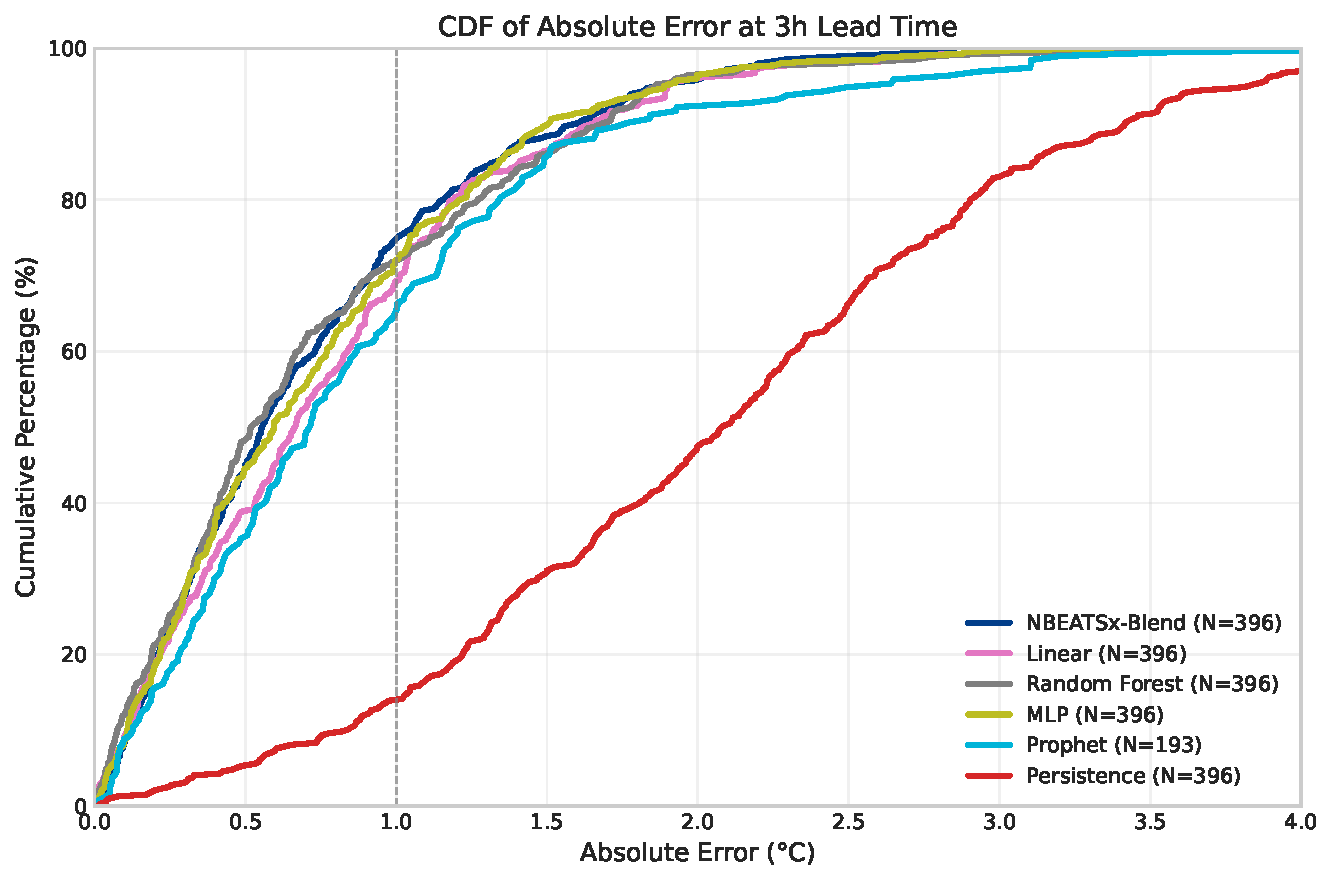
\includegraphics[width=\textwidth]{fig5_cdf_error.pdf}
    \caption{Forecast error distributions at the 3\,h dome-opening lead, evaluated on 396 twilights in 2025. \textbf{Left:} kernel density estimate of the signed residuals. \textbf{Right:} cumulative distribution of $|$error$|$, with the dashed line marking the 1\degC{} target. NBEATSx+Ridge achieves 80\% of predictions within 1\degC{}, versus 65\% for solar-persistence.}
    \label{fig:cdf}
\end{figure}

\subsection{Seasonal effects}
\label{sec:results:seasonal}

Forecast skill varies systematically with season. Figure~\ref{fig:seasonal_trends} splits the morning-forecast (9\,h lead) residuals by Southern-hemisphere season: Summer and Fall achieve low outlier rates ($|\text{residual}|>2$\degC{} in 7.4\% and 7.5\% of forecasts), while Winter and Spring are roughly twice as hard (19.6\% and 14.4\%). We trace this spread to a single underlying cause---day-to-day synoptic variability---rather than to any one class of weather event. The mean night-to-night change in twilight temperature grows from 1.1\degC{} in Summer to 3.2\degC{} in Winter---a seasonal rise in volatility visible directly in the full-year panel of Fig.~\ref{fig:dataset_overview}, where the winter months show the largest day-to-day swings of the year. This night-to-night change is the strongest correlate of the 9\,h error, and on changing nights the model systematically lags the trend (signed error correlated with the day-to-day change at $r\approx0.5$--$0.6$). Because these swings have little night-to-night persistence, they are largely irreducible from local temperature history alone, and they set the floor on long-lead seasonal performance.

Part of this gap is nonetheless recoverable from auxiliary local observations---humidity, wind, and multi-day temperature trends---supplied to the Ridge stage at long lead, where they reduce the 9\,h RMSE by 7.2\% in Winter (1.80 to 1.67\degC{}) and 5.4\% in Spring (1.61 to 1.53\degC{}) with no penalty at the operationally critical 3\,h lead. The Spring improvement is driven by humidity: humid evenings depart from the dry-climatology cooling curve the model has learned (the Atacama \emph{desierto florido} regime), an effect that is strongly nonlinear and concentrated at the morning lead. Wind contributes a complementary signal once resolved into components along and across the bimodal summit flow. We conclude that the seasonal difficulty is fundamentally meteorological---set by synoptic variability---but that targeted exogenous channels meaningfully sharpen the hardest morning forecasts, and that these gains will grow as the training archive accumulates more examples of the rare high-variability regimes.

\begin{figure}[htb!]
    \centering
    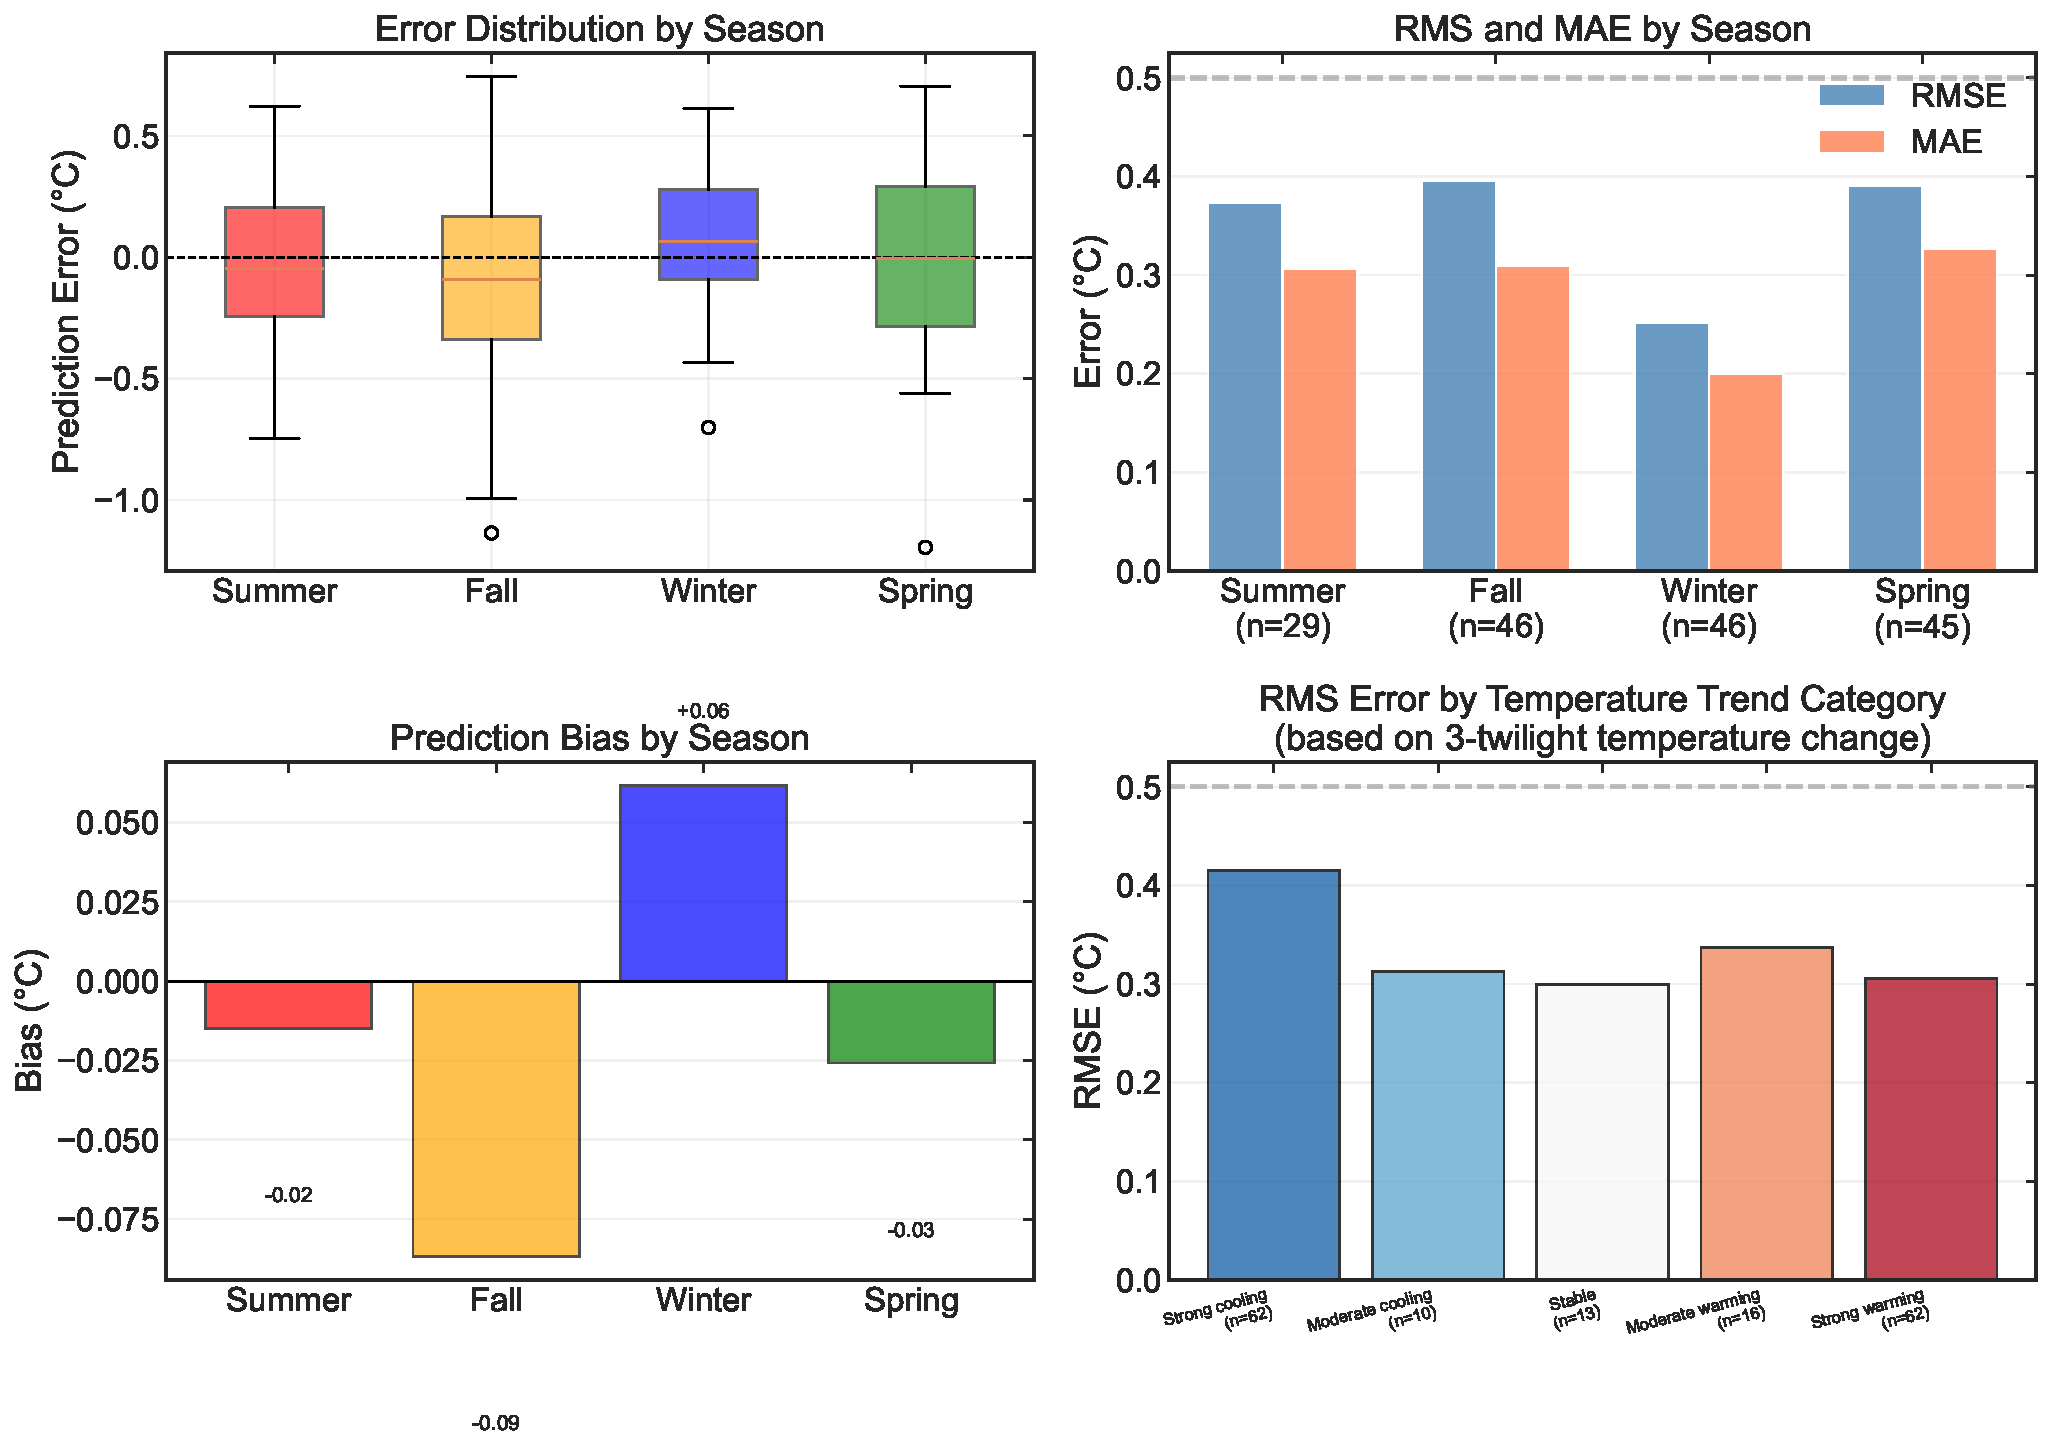
\includegraphics[width=\textwidth]{fig6_seasonal_trend_analysis.pdf}
    \caption{Morning forecast (9\,h lead) residuals split by Southern-hemisphere season. \textbf{Left:} kernel density estimate of the signed residuals. \textbf{Right:} CDF of $|$error$|$ with the inset listing the outlier rate $P(|\text{residual}|>2$\,\degC{}$)$ per season. Summer and Fall achieve low outlier rates (7.4\% and 7.5\%); Winter and Spring are harder (19.6\% and 14.4\%), driven by day-to-day synoptic variability that the model partially lags. The lead-gated trend, humidity, and direction-resolved wind features described in the text reduce the Winter/Spring morning-forecast error and are included in the results shown.}
    \label{fig:seasonal_trends}
\end{figure}

%% =============================================================
\section{DISCUSSION}
\label{sec:discussion}

\subsection{Two-stage architecture and Ridge stability}

The NBEATSx+Ridge architecture separates the forecasting problem into two complementary stages. NBEATSx, trained on the full pre-2025 contiguous solar-time grid ($\sim$20\,000 samples), learns nonlinear temporal dynamics from a small set of causal features (absolute temperature, 12\,h lag, trend slope, and 24\,h difference). Its direct-temperature prediction captures diurnal structure but carries a systematic bias that varies with atmospheric regime. The second-stage Ridge regression, trained on $\sim$430 pre-2025 twilight events, corrects this bias using a richer 13-feature set evaluated at the forecast issuance time, plus the NBEATSx prediction itself as the 14th input. The combination achieves 0.80\degC{} RMSE at the 3\,h dome-opening lead---a 6.5\% improvement over the best single-model baseline (Linear, 0.86\degC{}). Although NBEATSx ingests exogenous variables directly, it does not extrapolate them reliably to unseen atmospheric regimes; a lightweight linear correction evaluated at issuance time removes the residual systematic bias more effectively than folding the same features deeper into the network, which is why the Ridge stage adds disproportionate skill for its size.

We tested whether the Ridge stage benefits from online retraining as new 2025 data accumulates (expanding-window Ridge, retrained monthly). We find no benefit: the overall RMSE is 0.809\degC{} with expanding-window versus 0.805\degC{} with the fixed pre-2025 calibration---a negligible difference. The Ridge coefficients are already well-determined from $\sim$430 training twilights and transfer robustly to the 2025 test year without adaptation. In short, the Ridge stage gains little from larger or more frequent retraining once the calibration set spans a full seasonal cycle; we therefore recommend retraining only on an \emph{annual} cadence---enough to keep all four seasons represented as the archive grows.

\subsection{MeteoBlue NWP does not improve the forecast}

We evaluated a variant that ingests the bias-corrected MeteoBlue commercial NWP forecast (per-solar-time-bin slope-and-bias calibration, 48 bins) as either a future exogenous input to NBEATSx or a Ridge feature. In both configurations the NWP channel \emph{degrades} performance: adding it as a futr\_exog increases 3\,h RMSE by $\sim$12\%, and adding it to the Ridge feature set produces no improvement in the greedy forward sweep. The bias-corrected MeteoBlue forecast carries a residual scatter of 2.0--2.9\degC{} per solar-time bin---larger than the model's own error budget at short leads---so it injects more noise than signal. This site-specific result reflects the limited spatial resolution of global NWP models at Cerro Pach\'on's complex topography.

\subsection{Comparison with traditional ML}

All three supervised baselines (Linear 0.86\degC{}, MLP 0.90\degC{}, Random Forest 0.92\degC{} at 3\,h) perform comparably, reflecting the quality of the engineered features on the solar grid. The relationship between inputs and target is approximately linear at the 3\,h horizon, giving Ridge regression a slight edge due to its regularization and lower variance on the limited training set ($\sim$400 twilights). NBEATSx+Ridge improves over all baselines by combining the neural network's temporal modelling with Ridge's feature-driven bias correction.

The fact that the deep network only narrowly outperforms a linear fit today is a data-volume effect, not a modelling deficiency. NBEATSx is currently data-deficient: its training RMSE is significantly smaller than its test RMSE. Sweeping NBEATSx capacity and regularization (width 16--256, 1--3 blocks, batch 32--256, dropout 0--0.3), larger networks lower the training RMSE but raise the test RMSE---a train--test gap of up to $\sim$0.6\degC{} at 9\,h---and dropout only recovers the small network's performance. With $\sim$400 twilights the nonlinear structure is not yet identifiable, so a low-variance linear map is near-optimal. We adopt the deep-learning approach deliberately as a forward-looking choice: its error scales with data far faster than the linear model's (Sec.~\ref{sec:discussion:samplesize}), so as the LSST archive grows NBEATSx can learn the nonlinear, regime-dependent weather patterns a fixed linear model cannot represent.

\subsection{Forecast precision vs.\ training data volume}
\label{sec:discussion:samplesize}

Figure~\ref{fig:samplesize} shows how the NBEATSx+Ridge RMSE depends on the size of the training window. We start the window in January~2024 and grow it to the full pre-2025 archive. At each size we retrain NBEATSx on the first $N$ rows of the solar-time grid, refit the Ridge stage on the twilights inside that window, and evaluate on all 396 twilights in 2025.

At every lead time the RMSE falls steadily as data accumulate. The 3\,h forecast improves from $\sim$3\degC{} with three months of training to 0.80\degC{} with fourteen months. The 12\,h forecast improves fastest, because the network needs many seasonal examples to extrapolate that far ahead. A power-law fit to the last six points ($\log\text{RMSE} \propto \alpha \log N$) gives $\alpha = -0.12$ at 3\,h and $\alpha = -0.19$ at 12\,h. No lead has saturated.

The LSST survey began in January~2026. We extrapolate the fits to mid-survey (2031, $\sim$130\,000 samples) and to the full 10-year survey (2036, $\sim$220\,000 samples). The projections are:

\begin{center}
\begin{tabular}{lcccc}
\toprule
Lead & Test (2025) & Begin (2026) & Mid (2031) & Full (2036) \\
\midrule
3\,h  & 0.80\degC{} & 0.73\degC{} & 0.64\degC{} & 0.60\degC{} \\
6\,h  & 1.08\degC{} & 0.98\degC{} & 0.86\degC{} & 0.81\degC{} \\
9\,h  & 1.38\degC{} & 1.26\degC{} & 1.11\degC{} & 1.05\degC{} \\
12\,h & 1.65\degC{} & 1.44\degC{} & 1.15\degC{} & 1.04\degC{} \\
\bottomrule
\end{tabular}
\end{center}

These projections are optimistic, as they assume the power-law scaling continues without saturating---an assumption that longer archives will eventually break, once the model has seen enough of the rare high-variability synoptic nights (Sec.~\ref{sec:results:seasonal}) that dominate the long-lead error and the remaining error becomes intrinsically unpredictable from local observations.

\begin{figure}[htb!]
    \centering
    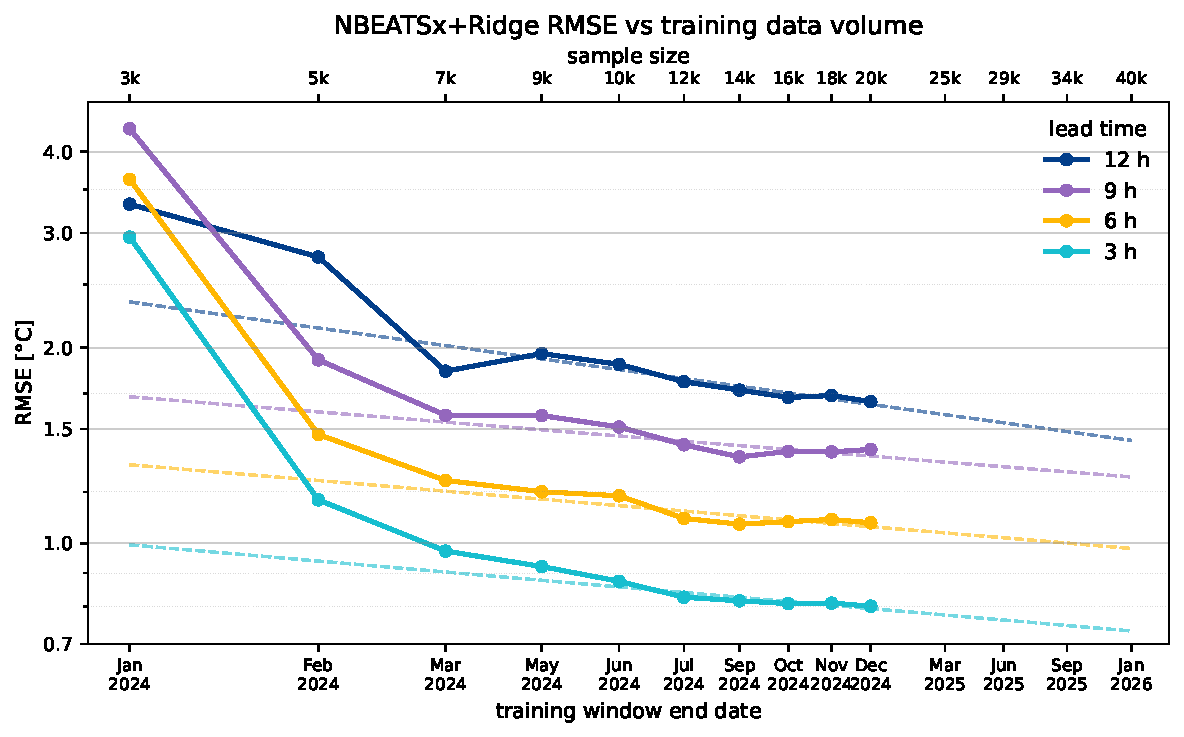
\includegraphics[width=\textwidth]{fig_rmse_vs_samplesize.pdf}
    \caption{NBEATSx+Ridge RMSE vs.\ training data volume, evaluated on 396 twilights in 2025. Solid lines: measured; dashed lines: power-law fit ($\log\text{RMSE} \propto \alpha\log N$, fitted to the last 6 points) extrapolated to the LSST survey start (January~2026). All leads continue to improve with accumulated training data. Top axis: training sample size in solar-grid rows; bottom axis: corresponding calendar date of the most recent training data.}
    \label{fig:samplesize}
\end{figure}

%% =============================================================
\section{LOOK-AHEAD THERMAL CONTROL OF RUBIN'S M1M3 MIRROR}
\label{sec:thermal}

With these temperature predictions in hand, we \emph{propose} a look-ahead thermal-control algorithm for Rubin's M1M3 mirror and evaluate it in simulation; the scheme has not yet been deployed at the observatory. During daytime (dome closed) the HVAC system controls dome-air temperature, while a forced-air circulation system drives temperature-regulated air into the mirror's hexagonal cells. For the purposes of this study we model the mirror temperature with first-order thermal dynamics,
\begin{equation}
\frac{dT_{\text{mirror}}}{dt} = \frac{T_{\text{setpoint}} - T_{\text{mirror}}}{\tau},
\label{eq:dynamics}
\end{equation}
adopting a representative thermal time constant $\tau = 3$ hours. Three constraints motivate the design: (i)~the mirror should be slightly cooler than ambient to avoid mirror seeing; (ii)~rapid setpoint changes induce spatial gradients and hex-cell print-through; (iii)~approaching the dewpoint risks condensation. We therefore target M1M3 at 1\degC{} below ambient during observations and adopt a soft controller capped at a 1.5\degC{}/hr maximum setpoint rate.

The proposed scheme sets the mirror temperature in three phases over the night (Fig.~\ref{fig:thermal_performance}). \emph{Daytime:} the dome is closed and the mirror is held at 1\degC{} below the forecast twilight temperature. \emph{Transition:} starting 3~hours before sunset, the setpoint ramps linearly from this daytime value to the nighttime law. \emph{Nighttime:} the setpoint follows the predicted ambient temperature, with a lead term that anticipates how fast it is changing,
\begin{equation}
T_{\text{setpoint}}(t) = \bar{T}_{\text{pred}}(t) + \tfrac{1}{2}\,\tau\,\frac{dT}{dt} - 1~^{\circ}\text{C}.
\label{eq:night}
\end{equation}
Here $\bar{T}_{\text{pred}}$ is the average predicted temperature over the next 3~hours (weighted toward the present), the $\tfrac{1}{2}\tau\,dT/dt$ term compensates for the mirror's thermal lag, and the $-$1\degC{} offset keeps it slightly cold. We assume the rate of change $dT/dt$ is known exactly (perfect knowledge); in practice it would be estimated from recent telemetry, a refinement we leave to future work. As an upper bound, we first run the controller with the \emph{true} future temperature. In this ideal case the mirror stays within $\pm$0.3\degC{} of its target for 82\% of the night (RMS scatter 0.26\degC{})---the best the scheme can possibly do.

We then repeat the simulation with the real forecast in place of the true temperature (Fig.~\ref{fig:thermal_performance}). The 3\,h forecast targets evening twilight, when the sun reaches $-20^\circ$ and the dome opens, about 80~minutes after sunset. This forecast sets the daytime and transition setpoint. From twilight onward, the mirror tracks the measured ambient temperature, and we score the error over the observing window. Across all 394 test nights (January 2025--January 2026), the forecast hits the twilight temperature to $-$0.04\,$\pm$\,0.40\degC{}, with 98\% of nights inside the $\pm$1\degC{} dome-opening tolerance. The mirror then stays within $\pm$0.3\degC{} of the target for 84\% of the night (RMS scatter 0.26\degC{}).

\begin{figure}[htb!]
    \centering
    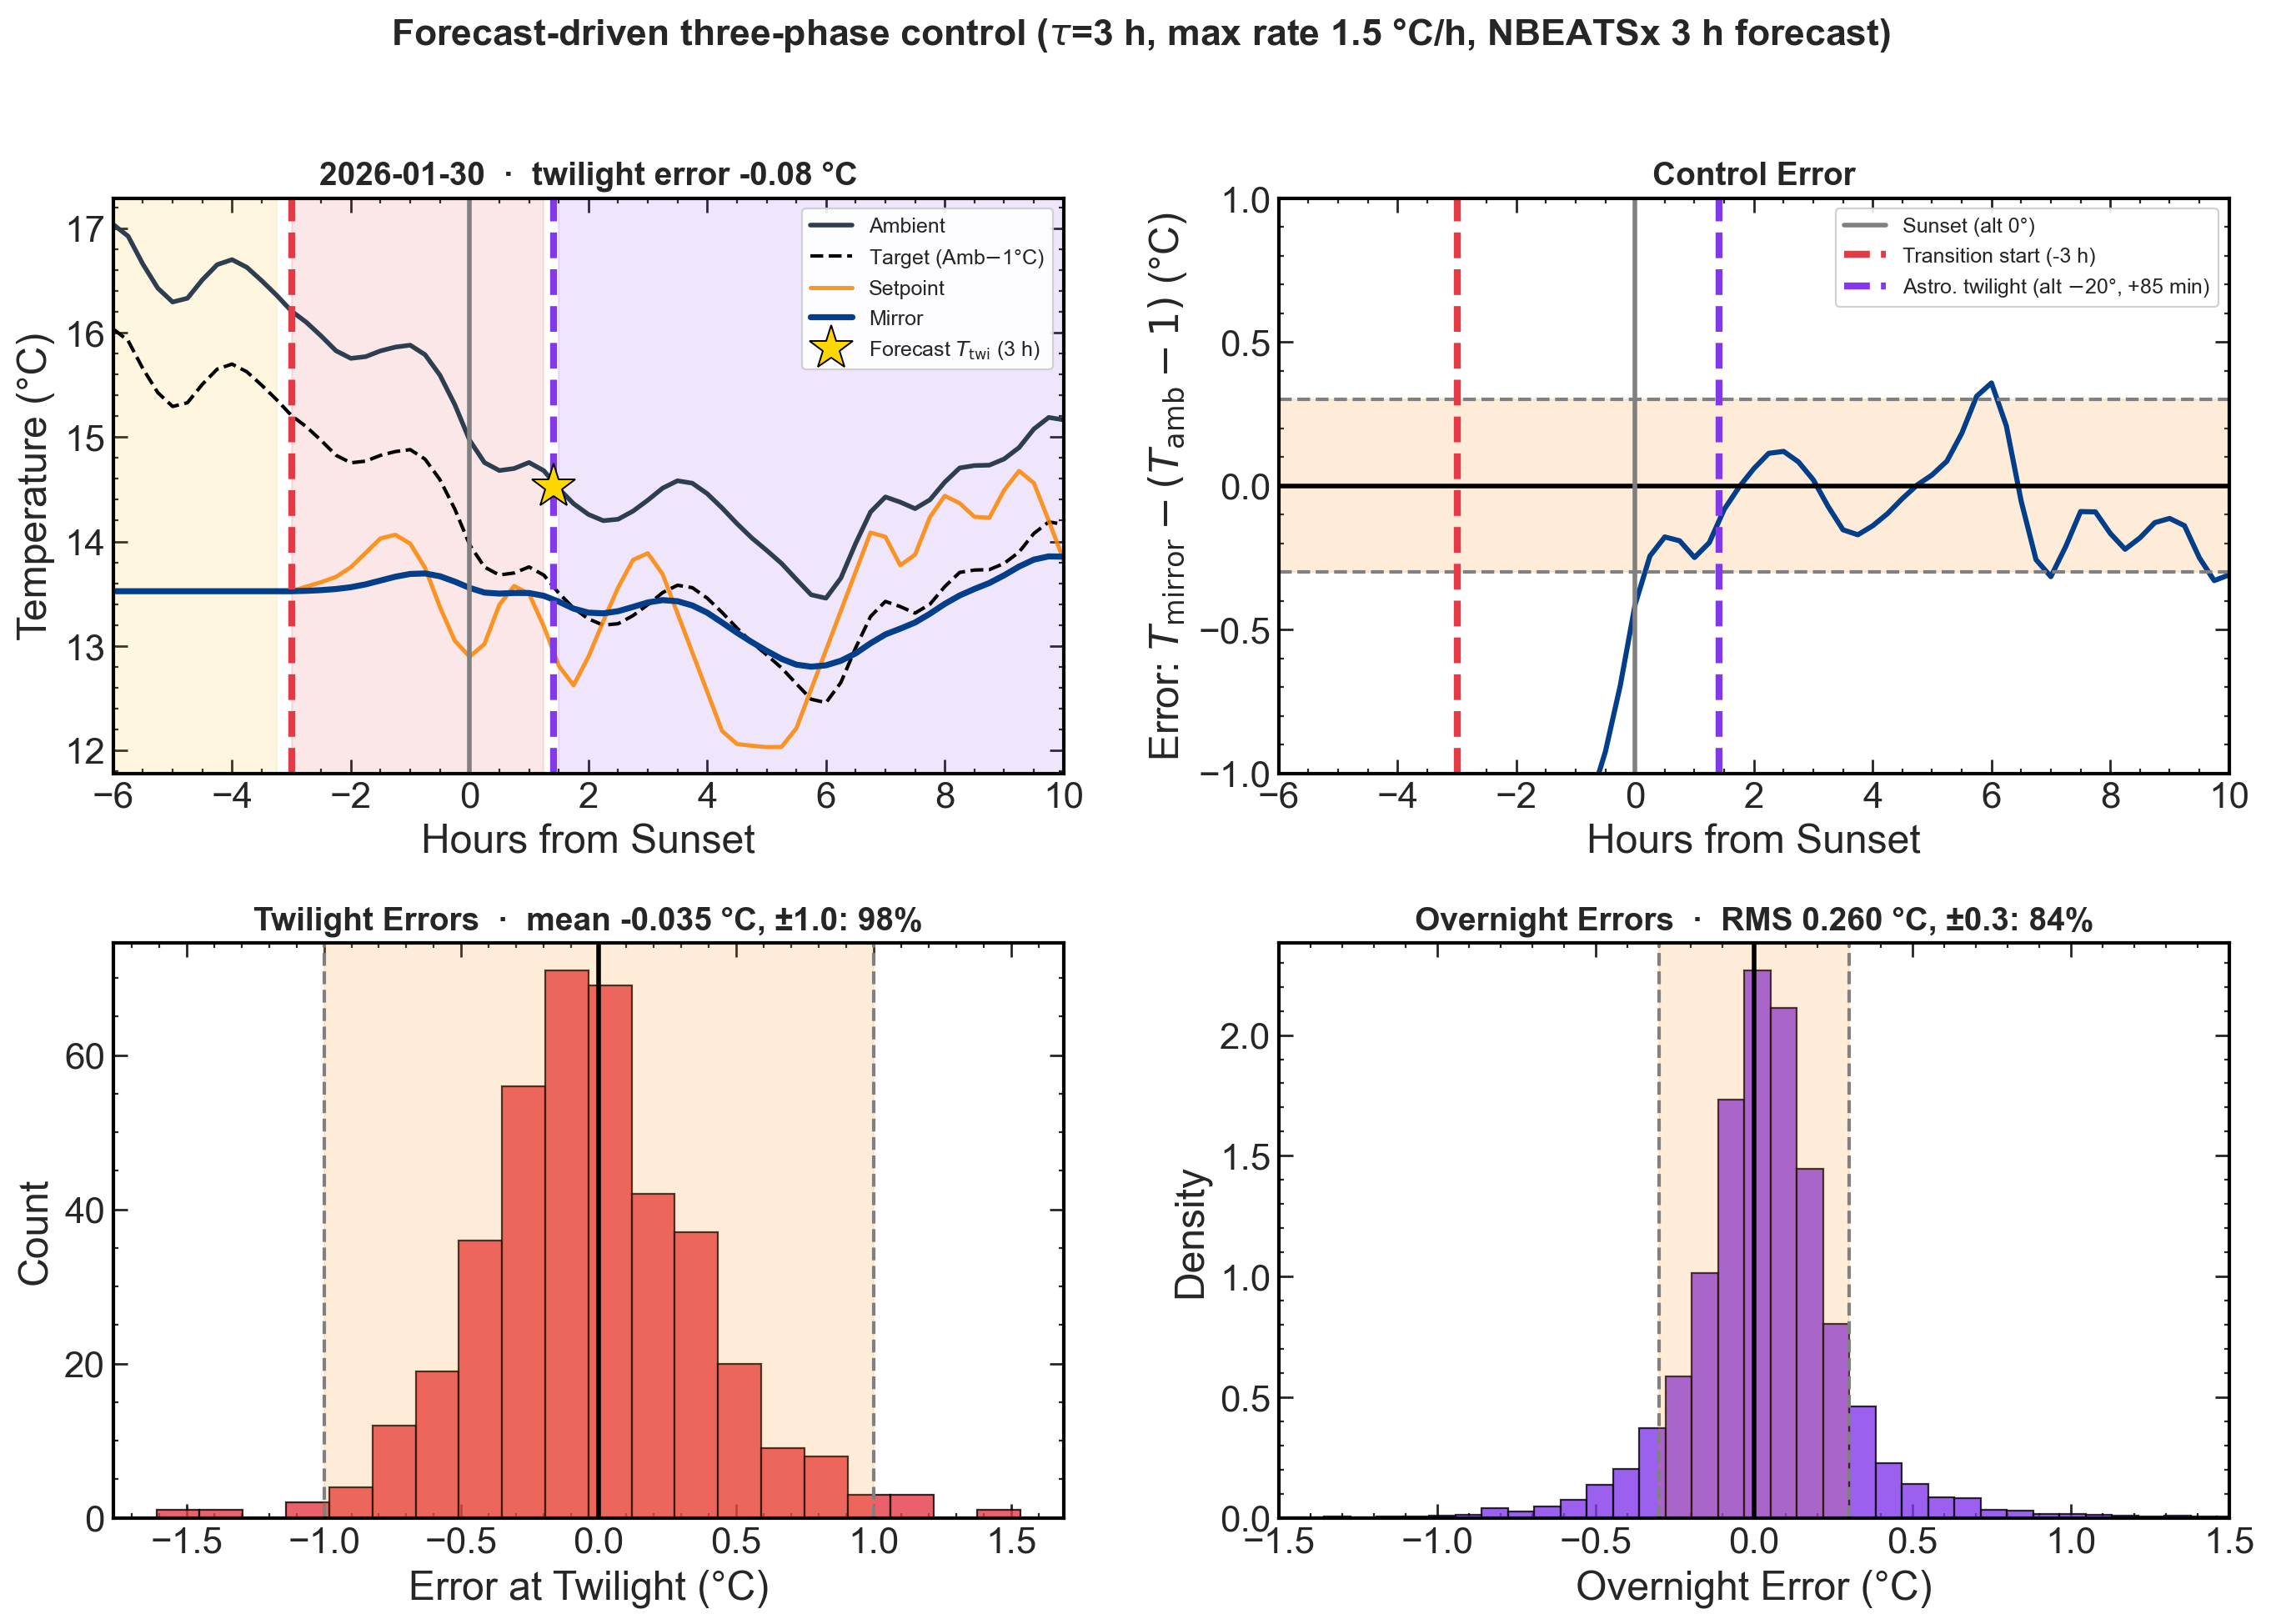
\includegraphics[width=\textwidth]{fig9_thermal_control.png}
    \caption{Proposed forecast-driven three-phase control, evaluated in simulation over all 394 test nights (January 2025--January 2026). \emph{Top left:} simulated temperature tracking on a representative clear night. The grey line marks geometric sunset (alt $0^\circ$), the red dashed line the transition start (3\,h before sunset), and the purple dashed line evening astronomical twilight (alt $-20^\circ$), where the overnight phase begins; shaded bands mark the three control phases. The NBEATSx 3\,h forecast of the twilight temperature (gold star) sets the daytime/transition setpoint, and the mirror (navy) follows ambient with the 1\degC{} cold bias overnight. \emph{Top right:} the corresponding control error stays within the $\pm$0.3\degC{} tolerance band (orange) through most of the observing window. \emph{Bottom:} twilight-error (counts) and overnight-error distributions across all test nights, with the $\pm$0.3\degC{} band shaded.}
    \label{fig:thermal_performance}
\end{figure}

At night the mirror simply follows the measured temperature, so the forecast matters most before the dome opens: it cools the mirror to the right starting point. A better twilight forecast means a smaller mirror--air gap at dome opening, which is when mirror seeing matters most. The forecast-driven and perfect-knowledge cases are statistically indistinguishable in overnight RMS (both 0.26\degC{}). The twilight forecast remains essential---it sets the mirror's starting temperature at dome opening---but reaching the ideal 0.26\degC{} RMS across the \emph{full} night would additionally require a short-term forecast that tracks the temperature \emph{during} the night, which we leave to future work. These results motivate an on-sky test. A real implementation would also need to handle the finite speed of the glycol and air actuators and the temperature gradients across the mirror, which our simple model in Eq.~\ref{eq:dynamics} leaves out.

%% =============================================================
\section{CONCLUSIONS}
\label{sec:conclusions}

We have presented NBEATSx+Ridge, a two-stage causal forecasting architecture for twilight temperature prediction at the Vera C. Rubin Observatory, and proposed a look-ahead thermal-control scheme that consumes these forecasts, evaluating it in simulation. Key findings:

\begin{enumerate}[noitemsep]
    \item NBEATSx+Ridge achieves RMSE of 0.80\degC{} at the 3\,h mirror-setpoint lead (80\% within 1\degC{}, 396 twilights in 2025); the bias-corrected MeteoBlue NWP retains $\sim$2\degC{} residual scatter at the site (Fig.~\ref{fig:comparison}).
    \item The two-stage design separates temporal modelling (NBEATSx, small network width=16) from feature-driven bias correction (Ridge, 13 features + the NBEATSx prediction). Neither stage alone matches the combined performance.
    \item Operating on a solar-time grid ensures twilight occurs at a fixed grid position regardless of season, making lag features physically consistent year-round; an ablation against an otherwise-identical clock-time grid shows this yields a mild ($\sim$6\%) RMSE improvement.
    \item We project a 3\,h RMSE of 0.73\degC{} at survey start (January~2026), 0.64\degC{} by mid-survey (2031), and 0.60\degC{} by the end of the 10-year LSST (2036), by extrapolating the power-law scaling of RMSE with training-data volume ($\text{RMSE} \propto N^{\alpha}$, $\alpha \approx -0.12$ at 3\,h).
    \item Commercial NWP (MeteoBlue) does not improve the forecast in any tested configuration: its bias-corrected residual scatter (2--3\degC{}/bin) exceeds the local model's error budget. The Ridge correction is stable without online retraining.
    \item In simulation, the proposed forecast-driven three-phase thermal-control scheme yields an ideal RMS scatter of 0.26\degC{} around the target of $T_{\text{M1M3}} - T_{\text{ambient}} = -1$\degC{}, maintaining M1M3 in the ideal range for 84\% of observing time---within 0.01\degC{} of the perfect-knowledge limit---motivating an on-sky trial.
\end{enumerate}

The NBEATSx+Ridge framework provides reliable, nearly unbiased temperature forecasts that improve autonomously as the observatory accumulates observing history. By the mid-survey epoch the 3\,h mirror-control setpoint forecast is projected to reach sub-0.7\degC{} precision---well within the thermal control system's tracking capability---enabling optimal image quality throughout the Legacy Survey of Space and Time. The same scaling projects the 9\,h morning forecast---which refines the daytime HVAC setpoint---to improve from 1.38\degC{} today to $\sim$1.11\degC{} by mid-survey (2031).

%% =============================================================
\acknowledgments

We sincerely thank our referees for their thorough review of this manuscript.
JHE and CWS are grateful for support from the DOE Cosmic Frontier program through grant DE-SC0007881, the Schmidt Science Foundation, and the Milton Fund at Harvard. Additional Rubin Observatory funding comes from private donations, grants to universities, and in-kind support from LSSTC Institutional Members. Anthropic's Claude Code tool was used extensively in the analysis presented here, and in the preparation of the manuscript and figures; all such outputs were carefully reviewed and verified by the authors.

%% =============================================================
\bibliographystyle{spiebib}
\bibliography{ref}

\end{document}
